\documentclass[12pt]{report}
\usepackage[utf8]{inputenc}
\usepackage{graphicx}
%\usepackage{algpseudocode}
\usepackage[boxed,vlined,linesnumbered,ruled]{algorithm2e}

\usepackage{tikz}
\usetikzlibrary{arrows,shapes}
\def\checkmark{\tikz\fill[scale=0.4](0,.35) -- (.25,0) -- (1,.7) -- (.25,.15) -- cycle;}
\tikzset{
  treenode/.style = {align=center, inner sep=0pt, text centered,
    font=\sffamily},
  arn_n/.style = {treenode, circle, white, font=\sffamily\bfseries, draw=black,
    fill=black, text width=2.5em},% arbre rouge noir, noeud noir
  arn_nc/.style = {treenode, diamond, white, font=\sffamily\bfseries, draw=black,
    fill=black, text width=2.5em},% arbre rouge noir, noeud noir
  arn_r/.style = {treenode, circle, red, draw=red, 
    text width=2.5em, very thick},% arbre rouge noir, noeud rouge
  arn_rc/.style = {treenode, diamond , red, draw=red, 
    text width=2.5em, very thick},% arbre rouge noir, noeud rouge
  arn_x/.style = {treenode, rectangle, draw=black,
    minimum width=0.5em, minimum height=0.5em}% arbre rouge noir, nil
}
\graphicspath{ {images/} }

\title{
	{Monte Carlo tree search applied to the game of Go}\\
	{\large UCL - Ecole polytechnique de Louvain}\\
	%{\includegraphics{university.jpg}}
}
\author{Vandermosten Thibault}
\date{Day Month Year}


\begin{document}

\maketitle


\chapter*{Abstract}

\chapter*{Dedication}

\chapter*{Declaration}

\chapter*{Acknowledgements}

\tableofcontents

\chapter{Introduction}
\section{start of intro}

\section{Rules of Go}

The rules of Go are extremely simple, and their simplicity allows a real complexity and depth of play. The game is played on go-ban, which are board of 9*9,13*13 or 19*19 intersections. There is two players, one who play the white stones, the other the black stones. Each player put a stone on an intersection on the go-ban alternatively.They are two important concept to understand, the liberties and the group. 
\\

A stone has as many liberties as free intersection next to it. In the following case, the black stone has initially four liberties, and it progressively decrease to one : 

\begin{center}
\includegraphics[scale=0.5]{Golibs}
\end{center}

Two or more stones can fusion together and form a group who share the liberties. Here we can see three group, one black and two white. The black one has five liberties by example. 

\begin{center}
\includegraphics[scale=0.5]{gogroupe}
\end{center}

An important concept is the capture, the board being representative(as a lot of ancient board games, like chess e.g) of a real situation of war. If a group is surrounded by the opponent, understand has no more liberties, it's dead. All the stones of the group are taken as prisoners, leaving the intersections where they were free. 

To win, you must have more point than your opponent. You gain one points by prisoner and one points by territory. A territory is a free intersection surrounded at least partially by your stones and potentially by the sides of the board. 

\begin{center}
\includegraphics[scale=0.4]{scorego}
\end{center}

\chapter{State of the art}

\textit{In this chapter, we will talk about what is Monte Carlo tree search (or MCTS) and how it is applied to Go.
First we will talk about the Monte Carlo part (2.1) and the tree search part (2.2) separately, then explain how the fusion works (2.3).
Then, in section 2.4, we will see the benefits and drawbacks as well as a dilemma in MCTS, exploitation versus exploration. 
And last but not least,we will see the application of MCTS to Go and which are some of the state of the art heuristics. }

\section{Monte Carlo and Tree search}

\subsection{Monte Carlo}

Monte Carlo methods are a big set of algorithms that works by using a repeated random sample to estimate a solution. They are widely used in a lot of domains like Physics, computational biology, computer graphics, computer science, Artificial intelligence,and even economics. 
\\

The Monte Carlo Method works by sampling enough data to estimate with enough precision a value. By example, if it seeks the mean between zero and one, it samples a lot of value between 0 and 1 and find the mean of all this values. With sufficiently high number, it will tends to 0.5. 

There are four steps in a Monte Carlo algorithm : 

\begin{itemize}
\item 1 : Define a domain that will contain all the possible values 
\item 2 : Sample random values over the domain following a probability distribution. It stops when there are enough value according to the level of precision required. 
\item 3 : Using the data sampled, it can compute results using theses values. 
\item 4 : With the results found, we can deduce other variable of importance using equations or theorems(depending of the domain of application). 
\end{itemize} 

We'll show this four steps through an example : the computation of $\pi$. How to estimate $\pi$ with a random generation Monte Carlo method. 

\begin{itemize}
\item Define a domain of inputs : the square of coordinates (-1,-1),(-1,1),(1,1) and (1,-11).
\item Generate random value over the domain following a probability distribution : Generate points following a uniform distribution in the square. 
\item Compute the result : compute $x$ where $x = \frac{In}{Total}$ and where $Total$ is the number of points sampled and $In$ is the number of points which fall within the circle of radius 1. 
\item Use the result to get what you wanted : With a sufficient high number of $Total$ we can approximate $\pi$ thanks to the law of big numbers and assuming


$$\frac{In}{Total}= \frac{\textrm{area of the circle}}{\textrm{area of the square}}$$

 As the area of the circle is $ \pi*1^2$ ,and the area of the square is $2*2=4$. And so we got our final approximation : 

$$
\frac{In}{Total}=\frac{\pi}{4}
$$
\end{itemize} 

Results have shown that with enough sampled values, it can get really close to the real value of $\pi$. 
\begin{figure}
\begin{center}
\includegraphics[scale=0.5]{circleMC}
\end{center}
\caption{Monte Carlo $\pi$ estimation}
%https://upload.wikimedia.org/wikipedia/commons/thumb/b/b0/MonteCarloIntegrationCircle.png/220px-MonteCarloIntegrationCircle.png
%TODO
\end{figure}
\subsection{Tree search}
In this section we explain the basics of tree search in artificial intelligence, some techniques already used and how they differ from MCTS. We present notably the mini max algorithm which is widely use in Artificial intelligence to show how his behaviour really differ from MCTS. 
\\

A tree is an abstract representation of a game. Each node represents a state of the game. The root is the initial state. Then there is one children for each move possible since that state. 
\\

Some assumptions need to be made : 
\begin{itemize}
\item The game is played turn by turn, not in real time. 
\item Two players.
\item Fully observable

\end{itemize}

Here's an example of a tree for a game where two players flip a coins and try to maximize the number of heads. The game begin with 0 heads for each player and the first to play is the red player. Either the coin is head then the game move to the node with 1 head or it's tail then the state is the 0 blue node. Then the black player plays and so on. The number in the node represent the number of heads since the beginning for the player of the same color as the node. 

\begin{center}
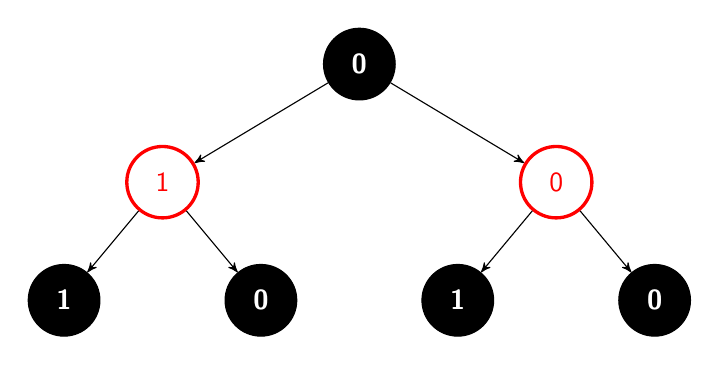
\begin{tikzpicture}[->,>=stealth',level/.style={sibling distance = 5cm/#1,
  level distance = 1.5cm}] 
\node [arn_n] {0}
    child{ node [arn_r] {1} 
            child{ node [arn_n] {1}}
            child{ node [arn_n] {0}}                            
    }
    child{ node [arn_r] {0} 
            child{ node [arn_n] {1}}
            child{ node [arn_n] {0}}                            
    }
; 
\end{tikzpicture}
\end{center}

\subsubsection{Mini-max}

The minimax algorithm is an algorithm used in artificial intelligence games. It gives to each state (or node) of the game a score. Then one player tries to maximize it while the other will try to minimize it. So a bigger score is a better situation for player one. Each action or move will impact the score. Thus, the algorithm chooses the action that eventually bring it into the best state for him, assuming the other player plays the best moves he can. If possible, the algorithm continue to search the tree until a won end game situation but as there is not always enough time, it limits itself to a certain depth. 
\\

Here is an example where the algorithm begin with the player looking to maximize the score and with a depth limit of two. 

At first, it doesn't know anything : 

\begin{center}
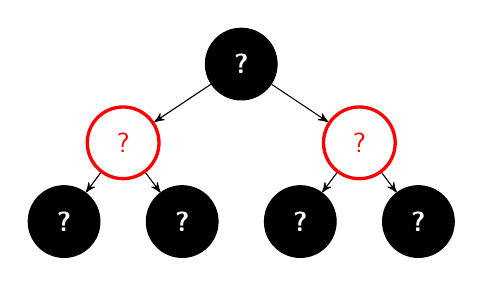
\begin{tikzpicture}[->,>=stealth',level/.style={sibling distance = 3cm/#1,
  level distance = 1cm}] 
\node [arn_n] {?}
    child{ node [arn_r] {?} 
            child{ node [arn_n] {?}}
            child{ node [arn_n] {?}}                            
    }
    child{ node [arn_r] {?} 
            child{ node [arn_n] {?}}
            child{ node [arn_n] {?}}                            
    }
; 
\end{tikzpicture}
\end{center}

Then it evaluates the value of the leaves. 

\begin{center}
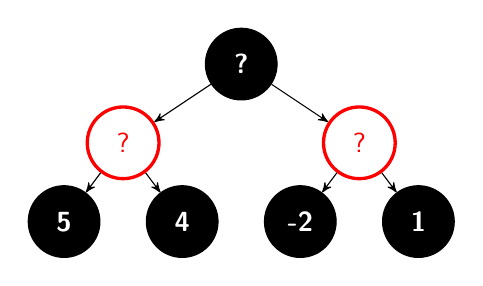
\begin{tikzpicture}[->,>=stealth',level/.style={sibling distance = 3cm/#1,
  level distance = 1cm}] 
\node [arn_n] {?}
    child{ node [arn_r] {?} 
            child{ node [arn_n] {5}}
            child{ node [arn_n] {4}}                            
    }
    child{ node [arn_r] {?} 
            child{ node [arn_n] {-2}}
            child{ node [arn_n] {1}}                            
    }
; 
\end{tikzpicture}
\end{center}

Then it computes the value for the red node, the player looking to minimize the score. So the algorithm assume that the player chooses at each time, the minimal node possible.

\begin{center}
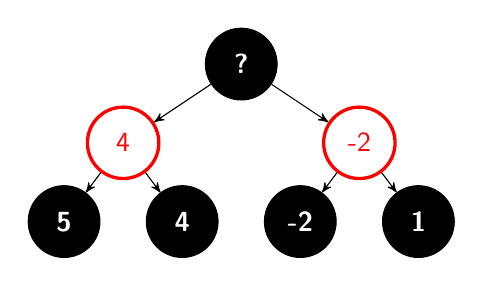
\begin{tikzpicture}[->,>=stealth',level/.style={sibling distance = 3cm/#1,
  level distance = 1cm}] 
\node [arn_n] {?}
    child{ node [arn_r] {4} 
            child{ node [arn_n] {5}}
            child{ node [arn_n] {4}}                            
    }
    child{ node [arn_r] {-2} 
            child{ node [arn_n] {-2}}
            child{ node [arn_n] {1}}                            
    }
; 
\end{tikzpicture}
\end{center}

Finally, it finds the value of the root node.
\\
\begin{center}
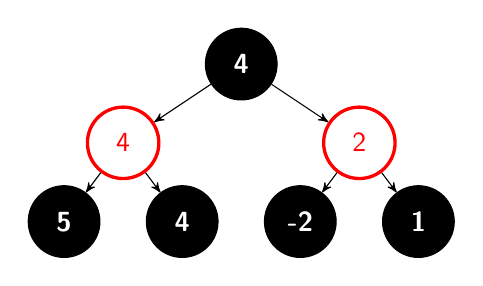
\begin{tikzpicture}[->,>=stealth',level/.style={sibling distance = 3cm/#1,
  level distance = 1cm}] 
\node [arn_n] {4}
    child{ node [arn_r] {4} 
            child{ node [arn_n] {5}}
            child{ node [arn_n] {4}}                            
    }
    child{ node [arn_r] {2} 
            child{ node [arn_n] {-2}}
            child{ node [arn_n] {1}}                            
    }
; 
\end{tikzpicture}
\end{center}

	
 This is the basis principle of a minimax search. There are several benefits to this technique but it suffers some major drawbacks. 
 
 \begin{itemize}
 \item It needs to explore in breadth first search, meaning all nodes from the top, depth after depth. In some case it's just impossible. The complexity of the minimax is $(b^d)*e$ where b is the branching factor(number of possible moves), d is the depth wished, and e is the complexity of the evaluate function. Example give : Go, the initial branching factor is 361 and the mean duration of a game is 200 plays.With such a complexity, $361^200$, it's impossible to compute the tree in reasonable time.
 \item The algorithm needs an evaluate function which return a value, a score for a node. It needs a deep knowledge of the game to produce a correct and precise heuristic when it's possible which is not always the case. In the case of Go, it's practically impossible to always being able give a value to a board, or even to say which player is at an advantage. The game can change on a single move. 
 \end{itemize}

\subsection{Monte Carlo and Tree search combined}

We now see how to combine these two principles to form the Monte Carlo tree search. The idea is relatively simple. As the total tree of the game is far to big, it only computes the necessary. Which means computing the tree node by node, with information on what nodes build next. And in the end, there is a far smaller tree indicating the best moves. In the following sections, the process for building the tree is detailed. 

\subsubsection{Four Steps}
This section presents how one execution of the Monte Carlo tree search occurs, through the four steps. Two names are given each time for the steps, it doesn't mean something different. It's just that theses steps are not called the same everywhere. The two names found were put to help a reader. We begin with a tree already partially built(\ref{Tree}. There's two colors, one for each player. The first number in the nodes is the number of times the owner of the root node won passing by that state. The second is the number of times the algorithm passed by that state. Example given the leftmost leaf, where see the red player won zero times on two tries. 
\begin{figure}
\begin{center}
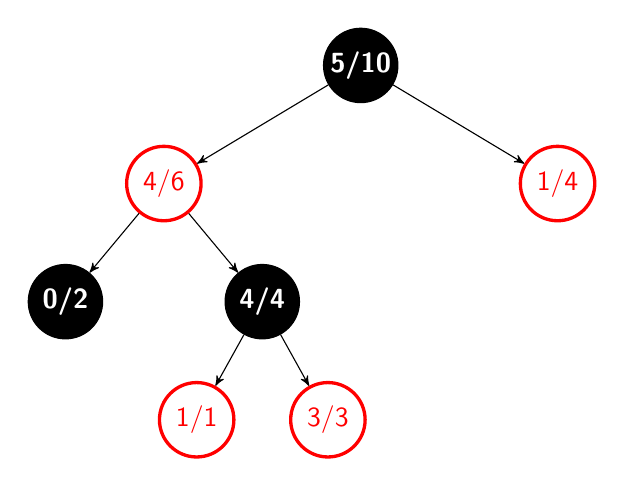
\begin{tikzpicture}[->,>=stealth',level/.style={sibling distance = 5cm/#1,
  level distance = 1.5cm}] 
\node [arn_n] {5/10}
    child{ node [arn_r] {4/6} 
            child{ node [arn_n] {0/2}}
            child{ node [arn_n] {4/4}
							child{ node [arn_r] {1/1}}
							child{ node [arn_r] {3/3}}
            }                            
    }
    child{ node [arn_r] {1/4}}
; 
\end{tikzpicture}
\end{center}
\caption{MCTS tree}
\label{Tree}
\end{figure}
\subsubsection{Selection(descent)}
The first step is the selection, the algorithm selects the best node following a criteria until a leaf is reached. This criteria can vary, and the different strategies will be explain further. For the moment, it simply is the one with the best ratio won over played. The chosen moves are highlighted in a diamond shape( \ref{Selec}). 
\begin{figure}
\begin{center}
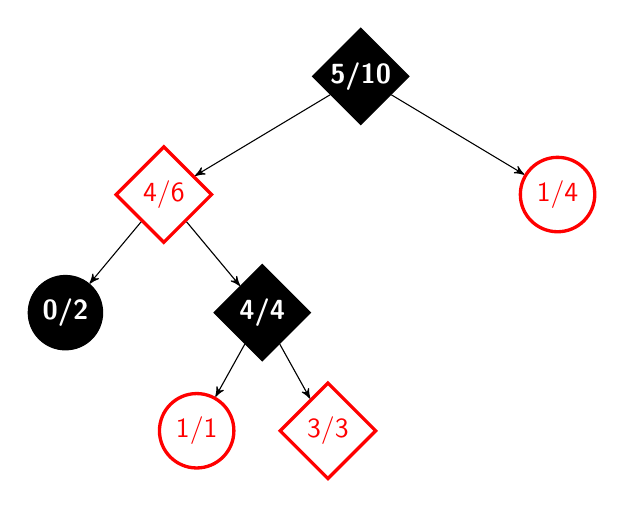
\begin{tikzpicture}[->,>=stealth',level/.style={sibling distance = 5cm/#1,
  level distance = 1.5cm}] 
\node [arn_nc] {5/10}
    child{ node [arn_rc] {4/6} 
            child{ node [arn_n] {0/2}}
            child{ node [arn_nc] {4/4}
							child{ node [arn_r] {1/1}}
							child{ node [arn_rc] {3/3}}
            }                            
    }
    child{ node [arn_r] {1/4}}
; 
\end{tikzpicture}
\end{center}
\caption{Selection step}
\label{Selec}
\end{figure}
\subsubsection{Expansion(growth)}
Once the selection phase reaches a leaf node of the tree built, it is the turn of the expansion phase.If the leaf is not a terminal state of the game, the basic strategy is to select a random move and add it to the tree with null statistics (\ref{Exp}).
\begin{figure}
\begin{center}
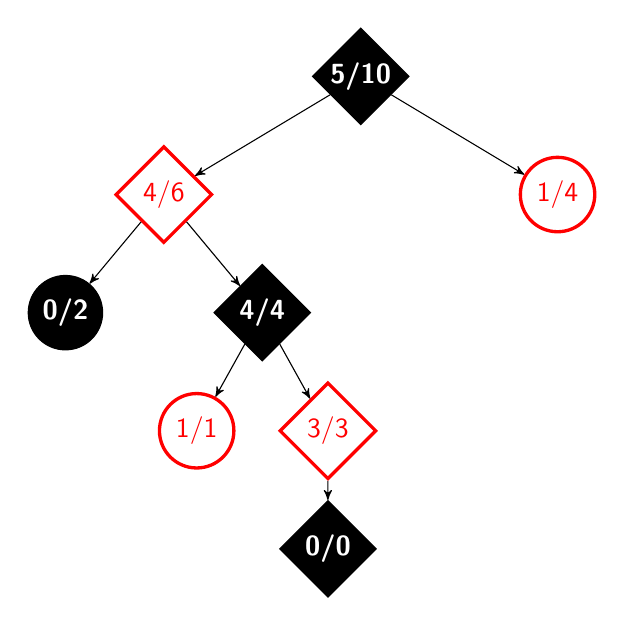
\begin{tikzpicture}[->,>=stealth',level/.style={sibling distance = 5cm/#1,
  level distance = 1.5cm}] 
\node [arn_nc] {5/10}
    child{ node [arn_rc] {4/6} 
            child{ node [arn_n] {0/2}}
            child{ node [arn_nc] {4/4}
							child{ node [arn_r] {1/1}}
							child{ node [arn_rc] {3/3}
								   child{ node [arn_nc] {0/0}}							
							}
            }                            
    }
    child{ node [arn_r] {1/4}}
; 
\end{tikzpicture}
\end{center}
\caption{Expansion}
\label{Exp}
\end{figure}

\subsubsection{Simulation(roll-out)}
The simulation steps plays until the end of the game with random possible move for both players. 

\subsubsection{Backpropagation(update)}
Once a final state is reached, it computes who's the winner and then, node by node, update the value of the tree. In the example, the black player will win. It will then update all the nodes on the path from the leaf node to the root. 


Once the game is ended, the algorithm computes the winner. Once done, it can update the nodes on the path taken, depending of the result. In the example, black won, so the values of all the diamond nodes will be updated accordingly (\ref{Back}). 
\begin{figure}
\begin{center}
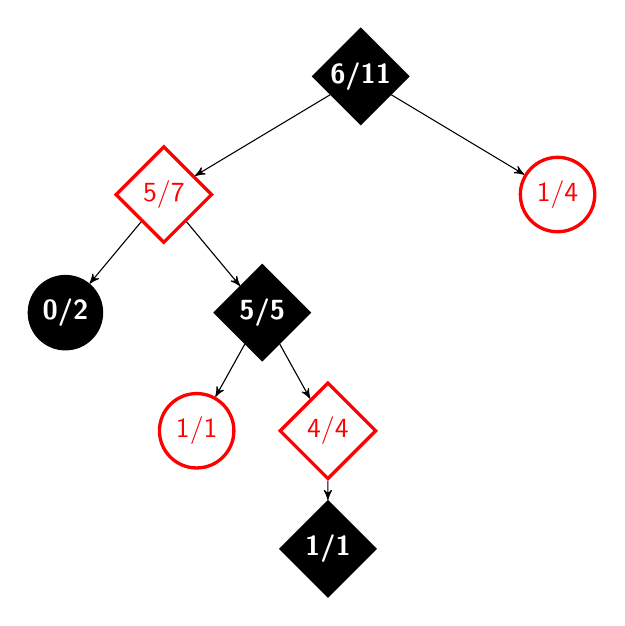
\begin{tikzpicture}[->,>=stealth',level/.style={sibling distance = 5cm/#1,
  level distance = 1.5cm}] 
\node [arn_nc] {6/11}
    child{ node [arn_rc] {5/7} 
            child{ node [arn_n] {0/2}}
            child{ node [arn_nc] {5/5}
							child{ node [arn_r] {1/1}}
							child{ node [arn_rc] {4/4}
								   child{ node [arn_nc] {1/1}}							
							}
            }                            
    }
    child{ node [arn_r] {1/4}}
; 
\end{tikzpicture}
\end{center}
\caption{Backpropagation}
\label{Back}
\end{figure}

The execution of one iteration is now finished. There is two possibilities, either there's still time, and the algorithm go on, or it ran out of time, and it must choose a move. In that case, it returns the a node following a criteria. With the criteria of the best ratio won over plays, it would return the move on the left. Indeed, by choosing that, it has 5 out of 7 chances to win, where in the other case, he would have less probability to win. 
\\

Thus, it's the principle of the Monte Carlo tree search. Only searching where it's interesting. By doing enough iterations, like with the computation of $\pi$, we can compute a tree that will be big enough to be statistically representative. 
\\

Now we will explore the different strategies possible for each steps. 

\subsection{Basic Strategies for each step}

There are several strategies for each step. To understand well the strategies for the selection step, it must be clear that there's a big dilemma in the application of Monte Carlo tree search. The problem is between two elements : Exploitation, which means taking profits of what you already know, and Exploration, which means go see elsewhere for better. When you exploit, you can't explore and reciprocally. So there's always that question : "Am I on the right path ? should I go further on it, or should I try something else". 
The following section, with the strategies for the selection step enlightens some answers. 

\subsubsection{Selection - Objective Monte Carlo}

The goal of this technique is to compute a fairness function for each move. It attributes a probability to each possible move and will then select randomly one, following the found probabilities. The fairness function reflects the balance between the exploitation and exploration.
\\

First the fairness function for each move $m$ is the following, where $n_p, n_m$ is the count of visit for the parent of m, for m respectively, PM is all the possible moves and U(x) is the urgency function of x. 
$$
f_m = \frac{n_p U(m)}{n_m \sum\nolimits_{j \in PM} U(j)}
$$

U(x) is a function that allows estimating if a move must be played. To be exact, it's : 
$$
U(m) = erfc(\frac{v_0 -v_m}{\sqrt{2}\sigma_m}
$$
$v_x$ is the value of the node x

0 is the best move. 

$\sigma_x$ is the standard deviation of x. The standard deviation for a discrete variable with the same chance for each value is : 

$$ 
\sigma_x 	= \sqrt{\frac{1}{N} \sum\limits_{i=1}^{N} (x_i-\mu_i)^2}
$$

TODO

\subsubsection{Expansion}
There exist strategies where there is more than one node added by expansion step to the MCTS tree, but as it didn't prove to be more effective, we will keep expanding only one node by iteration.

\subsubsection{Simulation}
For this step, there are several techniques that are more or less between two extremes :choose a move at random or with heuristics. 

\begin{tabular}{ccc}
    & Random & Heursitics \\
   Benefits & Speed & Reflect real play \\
   Drawbacks & Non representative & order of magnitude slower \\
\end{tabular}

\subsubsection{Backpropagation}

TODO

\subsubsection{Selection of the final move}
There are several methods to choose the move after the MCTS tree is built. 

\begin{itemize}
\item Select the move with the highest count of wins divided by the counts of visits known as Max child
\item Select the move with the highest visits count known as Robust child
\item Select the move with the both highest count ( wins and visits), known as Robust-Max child
\end{itemize}

\subsection{Benefits and Drawbacks}

\subsubsection{Benefits}

Monte Carlo tree search draws a lot of advantages from his special technique of using tree search and random simulations. 
\begin{itemize}
\item Aheuristic : There's absolutely no need for heuristic in the refined version of Monte Carlo tree search. All you need to know about the game is the possible moves from a state, and the winning situations for a player. Except that, which are the basic rules, you don't need to know how to play, to be a professional or having a really good vision of  the game to implement an artificial intelligence player.
\item Asymmetric : In place of having a gigantic tree, taking an incredible amount of space, there's only the needed tree, much much smaller than the complete one. As it's build only depending of the needs, it can be completely asymmetric. 
\item Any time. One of the beautiful part of the Monte Carlo tree search is that you don't need a specific amount of time. There always is an output. Some algorithms take a certain amount of seconds or minutes, then delivers an answer. Here, the algorithm can always, at any time return an answer. Of course, the more time given, the better the answer. But it allows to stop the search, either after a certain time or a number of iterations through the four steps. 
\item The basic version of Monte Carlo tree search can be implemented really simply. But his efficient adaptation to complex games is difficult. 
\end{itemize}

\subsubsection{Drawbacks}

Here's come the second part about the big dilemma talked sooner.  There are several difficult choices. By example if the simulation heuristic is too complicated, it will take too much time, leading to fewer iterations and so to not statistically representative results. On the other hand, if it's too simple, it won't reflect real plays and even with a lot of simulation, won't be representative. 

There are heuristics, added to the core method of MCTS, that improves dramatically the results. It will be explained in the next chapter. 

\chapter{MCTS applied to Go}
\input{chapters/chap1b}

\chapter{Naive version}
\input{chapters/chap2}

\chapter{Optimization}
\input{chapters/chap3}


\chapter{Conclusion}
%\input{chapters/conclusion}

\appendix
\chapter{Appendix Title}
%\input{chapters/appendix}
\end{document}